% ============================================================
%  Póster (70 x 100 cm) — ¿Cómo estimar el índice de Theil con la GEIH?
%  Usa las mismas figuras que el informe (fig_*.pdf) y los mismos paquetes.
%  Compilar: pdflatex -> biber -> pdflatex -> pdflatex
%  Overleaf: este archivo, references.bib, ur.png y fig_*.pdf deben estar en la
%  RAÍZ del proyecto. Menu > Main document = poster.tex.
% ============================================================
\documentclass{article}

\usepackage[T1]{fontenc}
\usepackage[utf8]{inputenc}
\usepackage[spanish,es-nodecimaldot,es-nolists,es-noshorthands]{babel}
\usepackage{amsmath}
\usepackage{newtxtext,newtxmath}   % Times, como el informe
\usepackage{icomma}
\usepackage{graphicx}
\usepackage{xcolor}
\usepackage{array,booktabs}
\usepackage{enumitem}
\usepackage[paperwidth=70cm,paperheight=100cm,margin=2cm]{geometry}
\usepackage{csquotes}
\usepackage[backend=biber,style=apa]{biblatex}
\addbibresource{references.bib}
\renewcommand*{\bibfont}{\pequeno}

\pagestyle{empty}
\setlength{\parindent}{0pt}
\setlength{\parskip}{0.5em}
\setlist{nosep,leftmargin=1.3em,itemsep=0.35em}

% ---------- Colores de la Universidad (los mismos de la presentación) ----------
\definecolor{urojo}{RGB}{166,25,46}
\definecolor{urgris}{RGB}{90,90,90}

% ---------- Tamaños de letra para 70 x 100 cm ----------
\newcommand{\texto}{\fontsize{26}{32}\selectfont}
\newcommand{\pequeno}{\fontsize{21}{26}\selectfont}

% ---------- Caja con título rojo y borde rojo ----------
\setlength{\fboxsep}{0.6cm}
\setlength{\fboxrule}{3pt}
\newsavebox{\contenido}
\newenvironment{caja}[1]{%
  \par\noindent
  \colorbox{urojo}{\parbox{\dimexpr\linewidth-2\fboxsep\relax}{%
    \color{white}\fontsize{38}{46}\selectfont\bfseries #1}}\par\nointerlineskip
  \noindent\begin{lrbox}{\contenido}%
  \begin{minipage}{\dimexpr\linewidth-2\fboxsep-2\fboxrule\relax}\texto}
  {\end{minipage}\end{lrbox}%
  \fcolorbox{urojo}{white}{\usebox{\contenido}}\par}

\begin{document}

% ============================================================
%  Encabezado
% ============================================================
\noindent\colorbox{urojo}{%
  \begin{minipage}[c]{\dimexpr\linewidth-2\fboxsep\relax}
    \colorbox{white}{
\includegraphics[height=5cm]{ur.png}}%
    \hspace{1.5cm}%
    \begin{minipage}[c]{0.8\linewidth}
      \color{white}
      {\fontsize{68}{78}\selectfont\bfseries ¿Cómo estimar el índice de Theil con la GEIH?\par}
      \vspace{0.5cm}
      {\fontsize{36}{44}\selectfont Comparación de cuatro estimadores y desigualdad del ingreso laboral en Colombia, 2018--2026\par}
      \vspace{0.6cm}
      {\fontsize{30}{36}\selectfont Gabriel Salcedo, Jerónimo Marín, Isaac Suarez y Santiago Velandia\\
       Estadística --- Universidad del Rosario, 2026\par}
    \end{minipage}
  \end{minipage}}

\vspace{1cm}

% ============================================================
%  Dos columnas
% ============================================================
\noindent
\begin{minipage}[t]{0.485\linewidth}

\begin{caja}{Pregunta}
  Con los mismos datos de una encuesta hay varias formas de estimar el índice de Theil, y elegir mal produce sesgo.

  \textbf{¿Cuál de cuatro estimadores del Theil tiene mejores propiedades con la GEIH? Con ese estimador, ¿cómo cambió la desigualdad del ingreso laboral entre 2018 y 2026, y qué la explica?}
\end{caja}
\vspace{0.4cm}

\begin{caja}{Hipótesis}
  \begin{description}[leftmargin=2.2em,labelindent=0pt]
    \item[H1] El estimador ponderado (A) es consistente y tiene el menor ECM cuando $n$ crece.
    \item[H2] En 2026 la educación explica más desigualdad que cada una de las otras dimensiones.
    \item[H3] La desigualdad fue menor en 2026 que en 2018.
  \end{description}
\end{caja}
\vspace{0.4cm}

\begin{caja}{Datos}
  \begin{itemize}
    \item GEIH del DANE, enero a junio de 2018 a 2026 (2020 no entra).
    \item Ocupados de 15+ años, remunerados, con ingreso positivo, en 24 departamentos.
    \item 130.000 a 161.000 personas por año (21,6 millones de ocupados).
    \item El peso de quien no reporta ingreso se reparte entre quienes sí.
  \end{itemize}
\end{caja}
\vspace{0.4cm}

\begin{caja}{El ingreso no es lognormal}
  \centering
  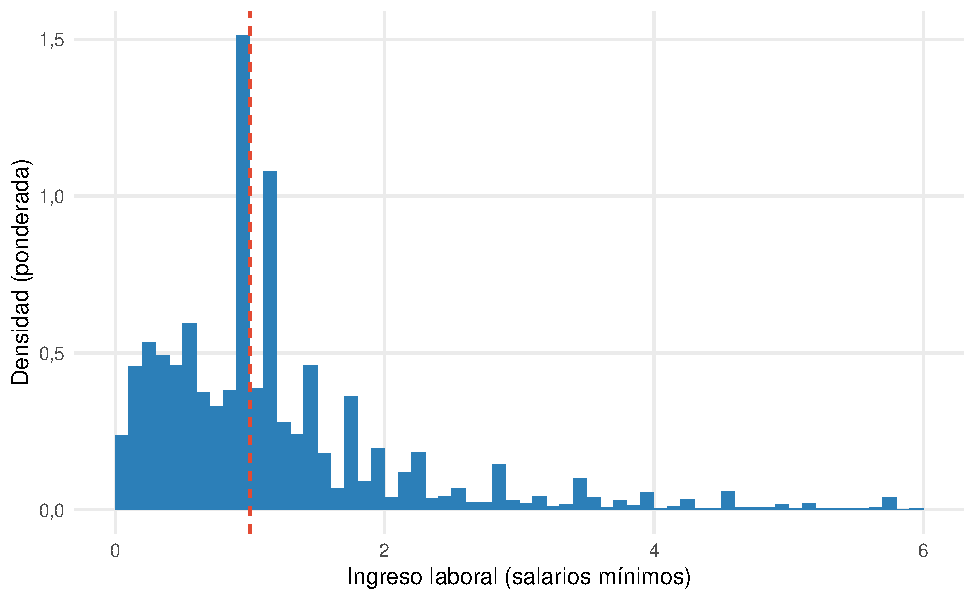
\includegraphics[width=0.6\linewidth]{fig_histograma_ingreso.pdf}

  \raggedright
  Pico en el salario mínimo: el 15,5~\% gana alrededor de un salario mínimo y el 39,5~\% gana menos. Por eso C y D fallan.
\end{caja}
\vspace{0.4cm}

\begin{caja}{Cuatro estimadores y la descomposición}
  \[ \hat T_A = \frac{1}{W}\sum_i w_i \frac{y_i}{\hat\mu_w}\ln\frac{y_i}{\hat\mu_w} \]
  \begin{itemize}
    \item \textbf{A:} con el factor de expansión $w_i$. \quad \textbf{B:} con $w_i = 1$.
    \item Si $\ln y \sim N(m,\sigma^2)$, entonces $T = \sigma^2/2$:
      \textbf{C} usa $\hat\sigma^2 = \ln(1 + CV^2)$ y
      \textbf{D} usa $\hat\sigma^2 = \frac{1}{n}\sum_i (\ln y_i - \overline{\ln y})^2$.
  \end{itemize}
  \[ T = \underbrace{\textstyle\sum_k s_k \ln(\mu_k/\mu)}_{\text{entre grupos}} + \underbrace{\textstyle\sum_k s_k T_k}_{\text{dentro de los grupos}} \]
\end{caja}
\vspace{0.4cm}

\begin{caja}{Simulación Monte Carlo: solo A es consistente}
  500 submuestras de la GEIH 2024 por cada $n$; referencia: $T = 0,5043$.

  \centering
  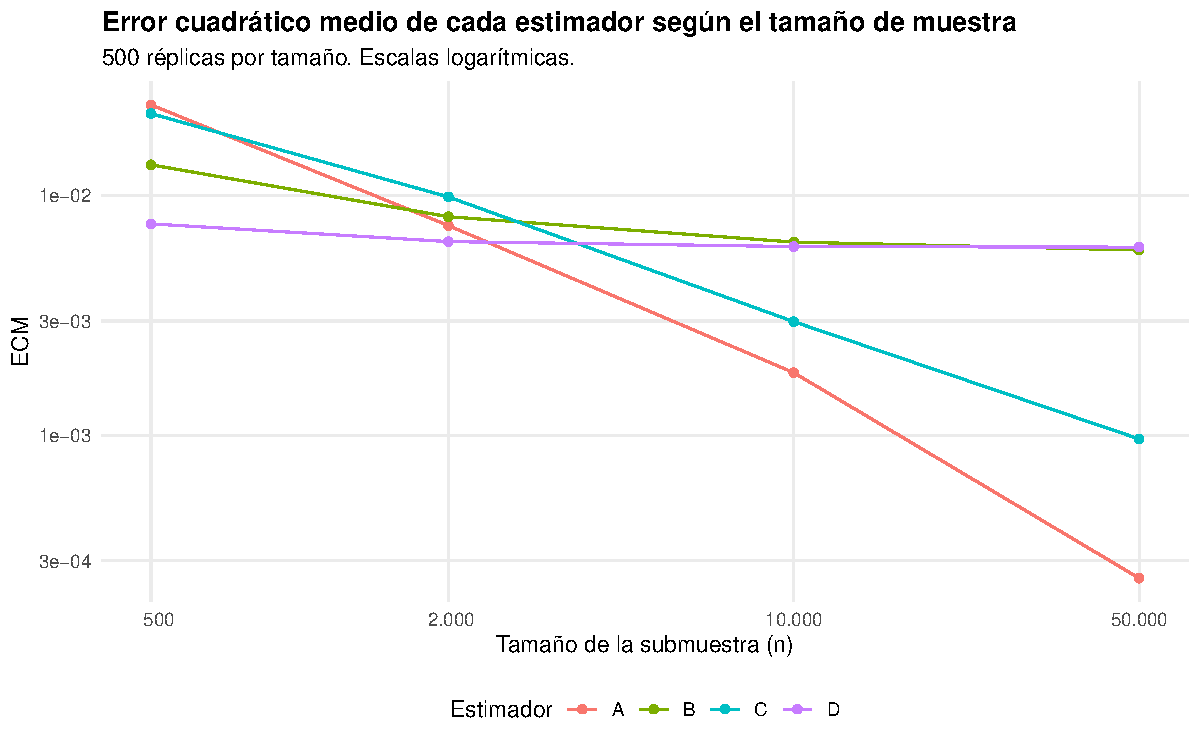
\includegraphics[width=0.65\linewidth]{fig_simulacion_ecm.pdf}

  \vspace{0.5cm}
  \begin{tabular}{@{}lrrr@{}}
    \toprule
    $n = 50.000$ & Sesgo & ECM $\times 1.000$ & ECM(A)/ECM(j) \\
    \midrule
    A (ponderado)       & 0,0003    & 0,25 & --- \\
    B (sin ponderar)    & $-$0,0766 & 5,93 & 0,04 \\
    C (lognormal, mom.) & 0,0243    & 0,97 & 0,26 \\
    D (lognormal, MV)   & $-$0,0780 & 6,09 & 0,04 \\
    \bottomrule
  \end{tabular}

  \raggedright
  \vspace{0.5cm}
  B y D subestiman la desigualdad en cerca de 15~\%; C la sobreestima en cerca de 5~\%.
\end{caja}

\end{minipage}%
\hfill
\begin{minipage}[t]{0.485\linewidth}

\begin{caja}{Desigualdad 2018--2026 (estimador A)}
  \centering
  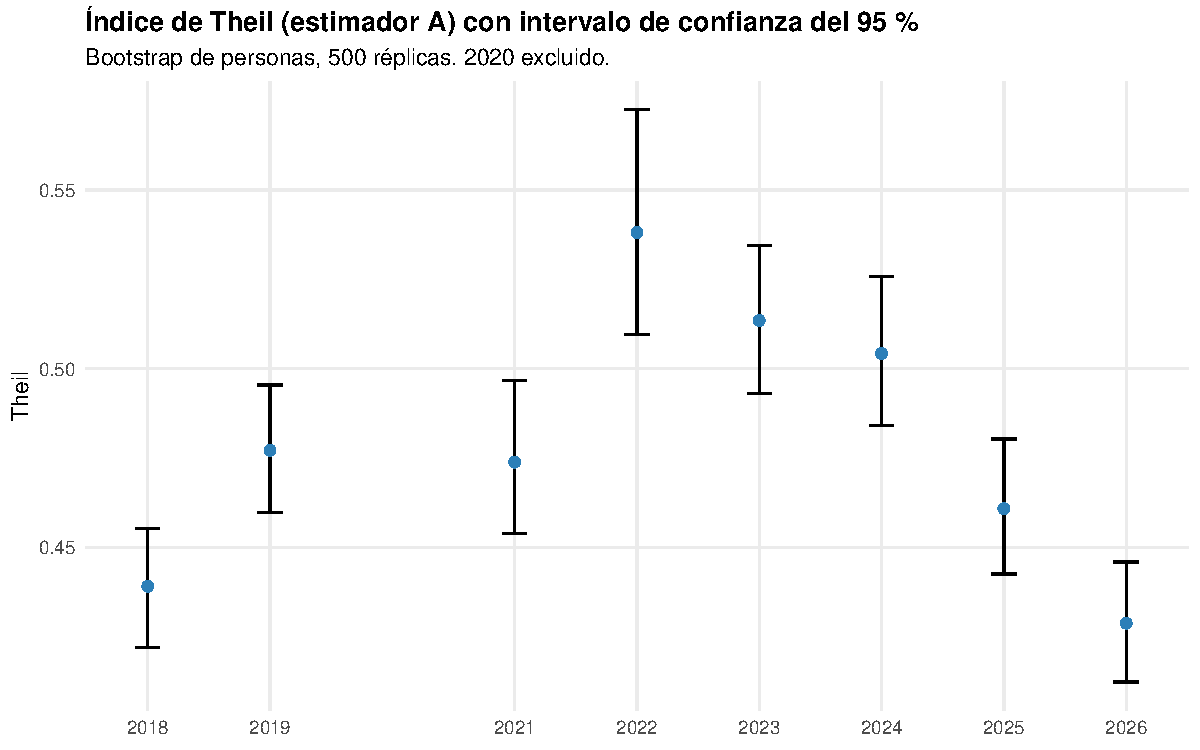
\includegraphics[width=0.9\linewidth]{fig_bootstrap_ic.pdf}

  \raggedright
  Intervalos bootstrap del 95~\% (500 réplicas). Máximo en 2022 (0,538), cuando cambió el marco muestral, y mínimo en 2026 (0,429).
\end{caja}
\vspace{0.4cm}

\begin{caja}{¿Qué explica la desigualdad?}
  \centering
  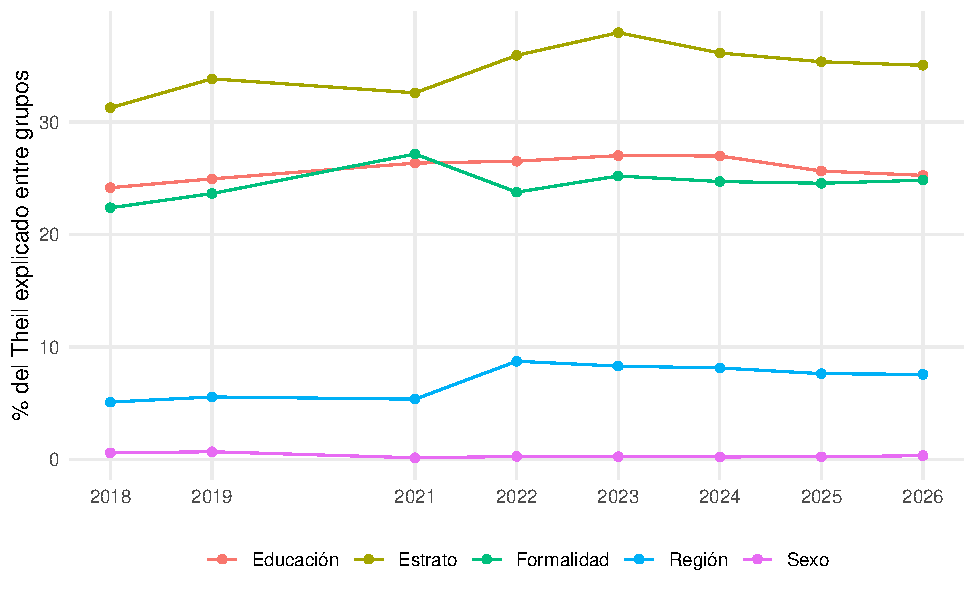
\includegraphics[width=0.9\linewidth]{fig_descomposicion.pdf}

  \raggedright
  El estrato explica entre 31 y 38~\% del Theil; la educación y la formalidad, entre 22 y 27~\%. La mayor parte de la desigualdad está \emph{dentro} de los grupos.
\end{caja}
\vspace{0.4cm}

\begin{caja}{Pruebas de hipótesis}
  \renewcommand{\arraystretch}{1.25}
  \begin{tabular}{@{}p{1.6cm}p{19.4cm}p{7.6cm}@{}}
    \toprule
    & Evidencia & Decisión \\
    \midrule
    H1 & $t$ pareada ($n = 50.000$): $p < 0,001$ frente a B, C y D & \textbf{Se rechaza $H_0$} \\
    H2 & La educación no supera a la formalidad ni al estrato & No se rechaza $H_0$ \\
    H3 & $T_{2026} - T_{2018} = -0,010$; percentil 95 $= +0,0085$ & No se rechaza $H_0$ \\
    \bottomrule
  \end{tabular}
\end{caja}
\vspace{0.4cm}

\begin{caja}{Conclusiones}
  \begin{itemize}
    \item \textbf{Con la GEIH hay que usar el estimador ponderado (A):} ignorar el factor de expansión o suponer lognormalidad produce sesgos que no desaparecen.
    \item La desigualdad subió hasta 2022 y bajó hasta su mínimo en 2026, pero la caída frente a 2018 no es significativa.
    \item El estrato es lo que más explica la desigualdad.
  \end{itemize}
\end{caja}
\vspace{0.4cm}

{\pequeno
  \nocite{theil1967economics,shorrocks1980class,cowell2011measuring,efron1993introduction,dane2026geih}
  \printbibliography[heading=none]
  \vspace{0.3cm}
  \color{urgris} Código y datos: \texttt{github.com/gabrielsalcedo/statistics-geih}\par}

\end{minipage}

\end{document}
